\chapter{基于轨迹单调性的\epsl{}判定}

在这一章节中,本文将先对Kim等人提出的\epsl{}\cite{kim2013stereoscopic}进行介绍,然后进一步阐述本文在此基础上进行的推导。

\section{\epsl{}}

\begin{figure}[tbh]
    \centering
    \subfloat[\epslb{}]{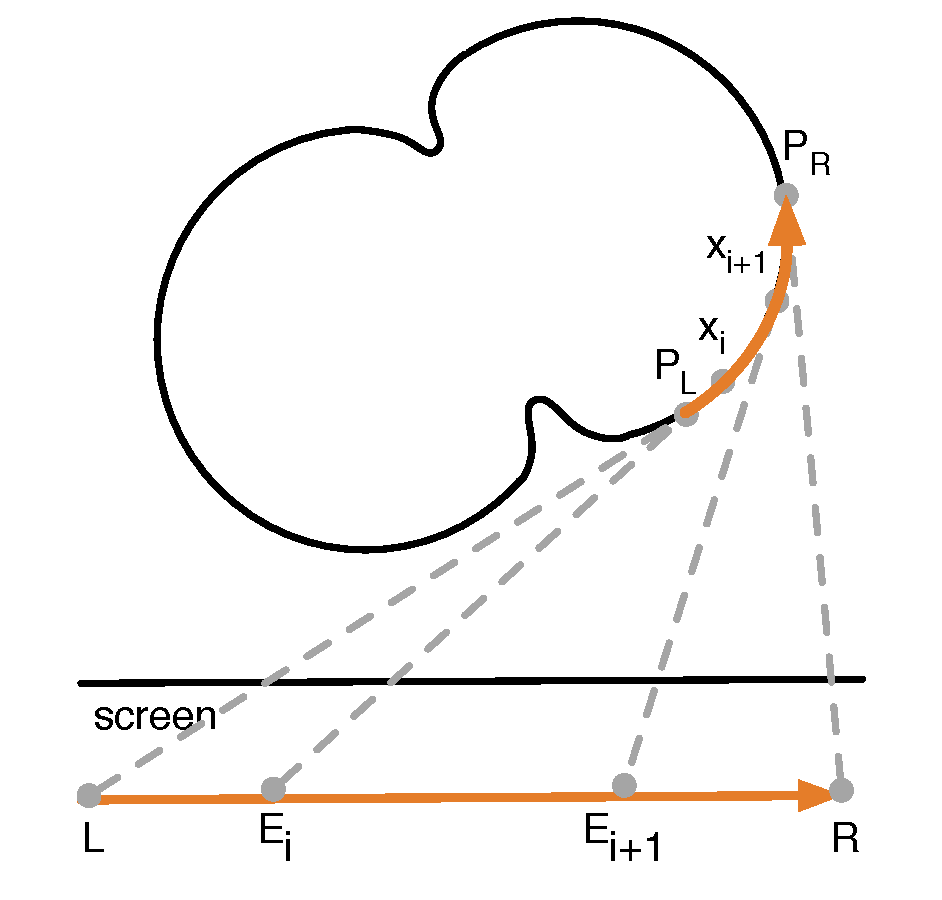
\includegraphics[width=.5\linewidth]{slidable}}
    \hfil
    \subfloat[不是\epslb{}]{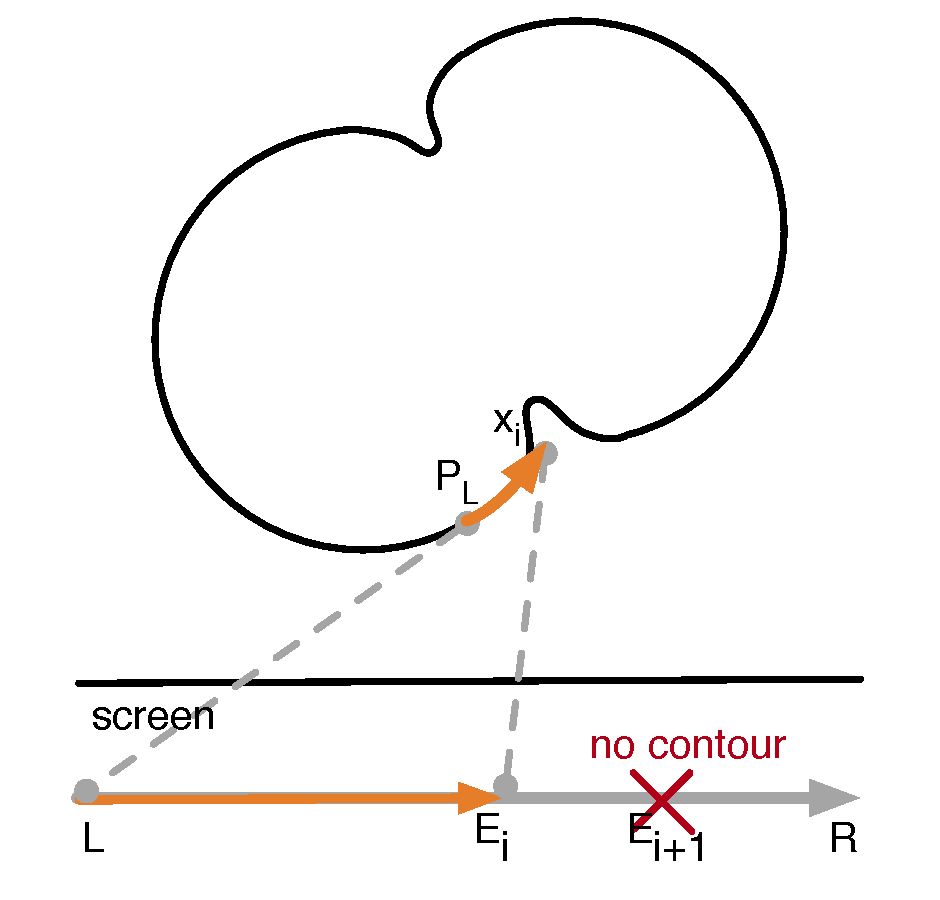
\includegraphics[width=.5\linewidth]{unslidable}}
    \caption[\epsl{}的定义]{\epsl{}的定义。(a)表示$P_L$是\epslb{},(b)表示$P_L$不是\epslb{}。} \label{fig_sim2}
    \label{fig:slidability}
\end{figure}

\begin{figure}[tbh]
    \centering
    \subfloat[\epslb{}]{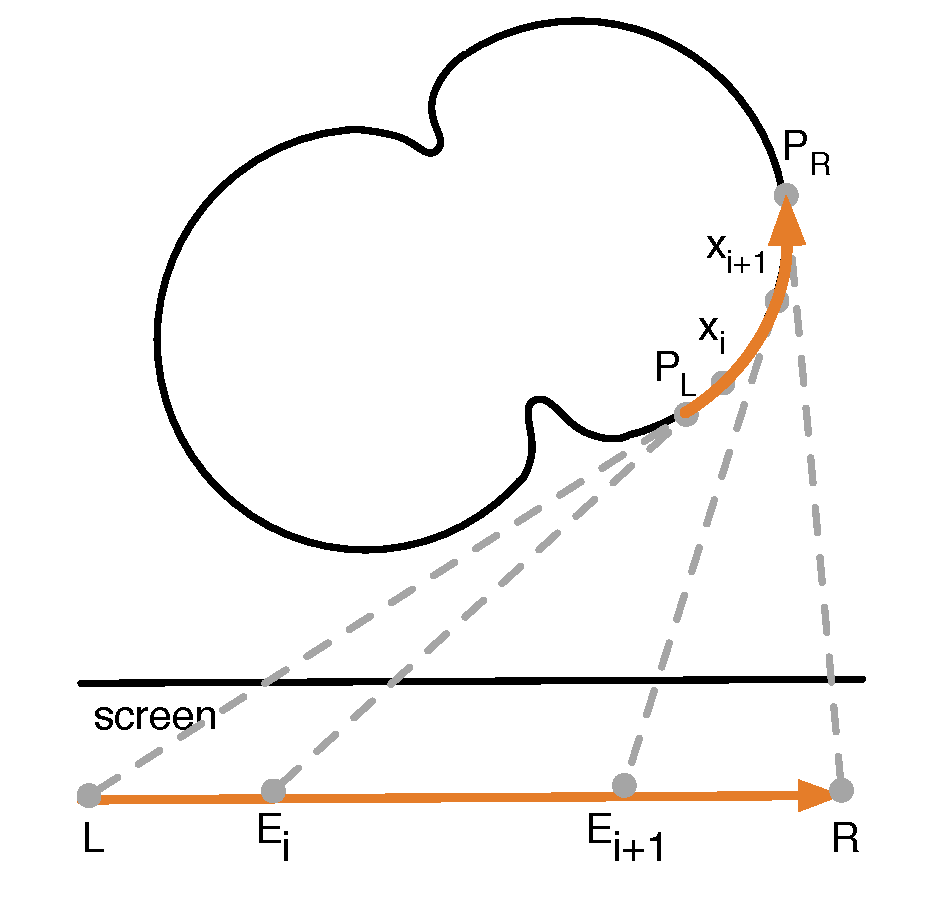
\includegraphics[width=.5\linewidth]{inverse_slidable}\label{fig:inverse_slidable}}
    \hfil
    \subfloat[不是\epslb{}]{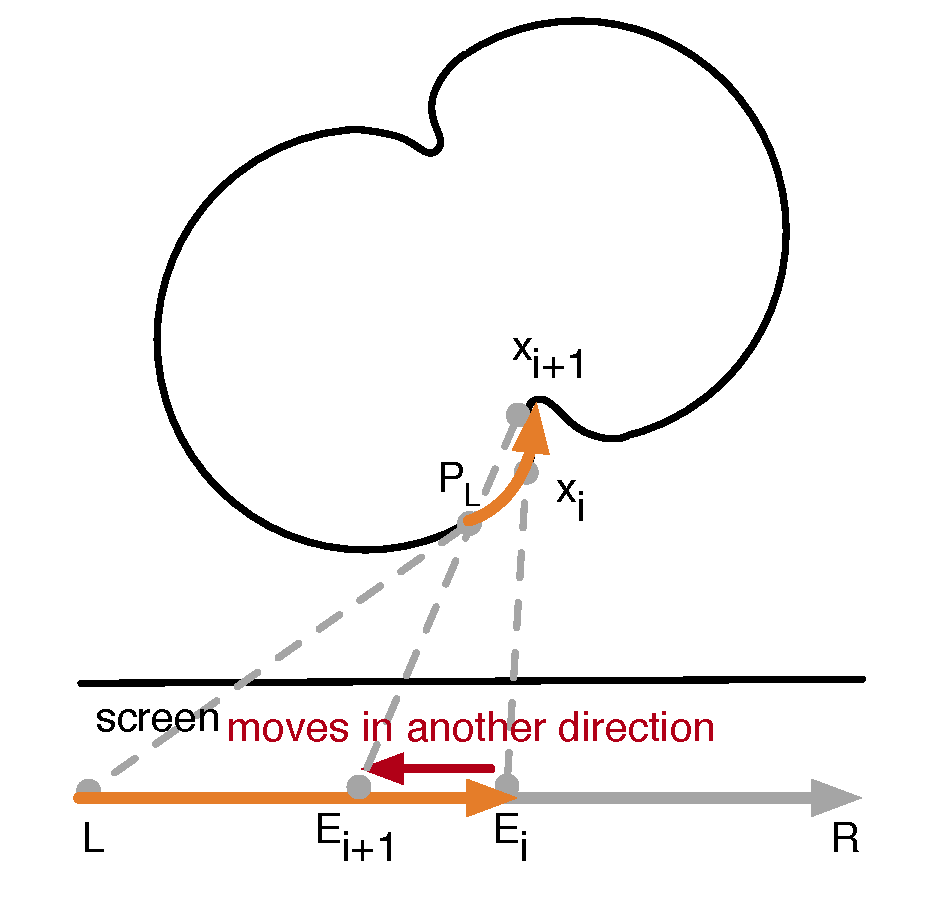
\includegraphics[width=.5\linewidth]{inverse_unslidable}\label{fig:inverse_not_slidable}}
    \caption[\epsl{}的推论]{\epsl{}的推论。(a)表示$P_L$是\epslb{},(b)表示$P_L$不是\epslb{}} \label{fig:inverse_slidability}
\end{figure}

以\con{}为例,如俯视图\autoref{fig:slidability}所示,\epsl{}的定义如下:假设$L$和$R$分别表示左眼和右眼对应的视点,$P_L$和$P_R$分别表示以$L$和$R$作为视点观察到的\con{}上的一个\conp{}。假设以$L$和$R$连线上的一个点$E$作为视点,当$E$从$L$向$R$移动,对应的轮廓点也应该从$P_L$向$P_R$移动,它在物体表面上移动的轨迹曲线${P_L}{P_R}$称为\ec{}\cite{geiger1995occlusions}。如果\ec{}上的轮廓点能够从$P_L$连续变化到$P_R$,那么$P_L$就是\epslb{}的(\autoref{fig:slidability}(a))。否则,如果\ec{}上的轮廓点能够从$P_L$连续变化到$P_R$,那么$P_L$不是\epslb{}的,不能和对应的轮廓点形成正确的立体视觉(\autoref{fig:slidability}(b)),因此该轮廓点应该在双目绘制的最终结果中被消去。
 
Kim等人在他们的工作上提出了一种对$P_L$的\epsl{}进行检验的方法。具体来说,他们的方法首先在两眼对应的视点$L$和$R$之间枚举多个视点$E_0$、$E_1$……$E_n$,并按照顺序在这些视点上基于三维模型的几何绘制出轮廓线。当所有相邻视点得到的轮廓点,例如\autoref{fig:slidability}(a)中的$E_i$、$E_{i+1}$分别得到的$x_i$和$x_{i+1}$,都满足$x_{i+1}$在$x_i$的\ec{}方向上的一定区间范围内,那么就$P_L$就是\epslb{}的轮廓点。简而言之,就是为了确定当$E$从$L$向$R$移动时对应的轮廓点也相应地从$P_L$向$P_R$移动,所以通过从$L$向$R$按顺序采样多个视点并绘制出轮廓线的图像来进行验证。

需要特别指出的是,虽然以上定义和方法使用\con{}为例进行表述,但是以上定义和方法对于\scon{}也同样成立,例如$P_L$和$P_R$也可以分别表示以$L$和$R$作为视点观察到的\scon{}上的一个\sconp{}。在下文的讨论中,本文也会先以\con{}为例进行表述,在有需要特别说明的情况下,再对\scon{}的情况进行特别说明。

\section{\epsl{}的推论}

前人提出的\epsl{}的概念已在上一小节进行了细致的说明,它对于\conp{}和\sconp{}在双目绘制的情况下是否应该被消去给出了明确的数学判定条件,具有重要的指导意义。本文提出的方法则拓展了\epsl{}的概念并提出了一个推论:要判定\epsl{},可以通过检查$P_L$到$P_R$的轮廓点的对应视点的轨迹来完成,从而避免在$L$和$R$之间采样多个视点所需要的繁重的计算,使得设计更加高效的\stc{}的\con{}和\scon{}绘制算法成为可能。

本文提出的方法的出发点如\autoref{fig:inverse_slidability}所示。假设一个\conp{}$x$沿着$P_L$到$P_R$的\ec{}移动,如果$P_L$是\epslb{}的,那么$x$对应的视点$E$会单调地从$L$移动到$R$(\autoref{fig:inverse_slidability}(a))。如果$P_L$不是\epslb{}的,那么对应的视点$E$不会在到达$R$之前保持一直朝着$R$移动(\autoref{fig:inverse_slidability}(b))。简单来说,本文上述的判定过程在本质上和Kim等人描述的\epsl{}的判定过程是一致是,只是本文是从\conp{}反推出视点的变化规律,并通过这个视点的变化规律来进行\epsl{}的判定,而不是像前人一样直接通过\conp{}的变化来进行\epsl{}的判定。

不难发现,以上提出的推论虽然以\con{}为例进行表述,但是对于\scon{}也完全适用。但是由于\con{}和\scon{}的数学定义不同,所以下面开始分别对\con{}和\scon{}用明确的数学语言给出有关\epsl{}的推论。

\subsection{\con{}}

基于上述的想法,对\epsl{}的判定可以转化为对对应视点的运动轨迹的单调性的判定。具体而言,假设有一个在\ec{}上移动的\conp{}$x$,对应的将$x$视为\conp{}的视点$E$可以用如下的公式计算:

\begin{equation}\label{eq:viewpoint2}
    {(E - P)}\cdot{N} = 0
\end{equation}

其中$P$和$N$分别表示\conp{}$x$的位置和法线方向,$E - P$表示视点$E$与$x$形成的视线方向。

又因为$E$位于$L$和$R$之间的连线上,所以它的位置可以用一个变量$t$进行以下的参数化:

\begin{equation}\label{eq:viewpoint1}
    E = (1-t)L+t R
\end{equation}

联立\autoref{eq:viewpoint2}和\autoref{eq:viewpoint1}可以得到:

\begin{equation}\label{eq:t1}
t = \frac{(P-L)\cdot{N}}{(R-L)\cdot{N}}
\end{equation}

\autoref{eq:t1}表示$t$是一个关于表面点$x$的函数。当$x$沿着\ec{}运动,$t(x)$就是轮廓点$x$的对应视点的轨迹函数。为了将\con{}和\scon{}对应的轨迹函数区分开来,本文使用$t_c(x)$来表示\conp{}的对应视点的轨迹函数,用$t_s(x)$来表示下文将要阐述的\sconp{}的对应的视点的轨迹函数,并用$t(x)$来对以上两种轨迹函数进行合称。

为了进一步讨论轨迹函数$t_c(x)$的单调性,本文将$t_c(x)$的导数形式计算如下:

\begin{equation}\label{eq:derivative}
    % \begin{split}
  t_c' = \frac{(P'\cdot{N}+(P-L)\cdot{N'})((R-L)\cdot{N})}{((R-L)\cdot{N})^2}-\frac{((R-L)\cdot{N'})((P-L)\cdot{N})}{((R-L)\cdot{N})^2}
    % \end{split}
\end{equation}

为了表达上的简洁,本文将\autoref{eq:derivative}中两边的$x$隐去。基于此公式,可以通过$t_c'(x)=0$找到极值点,从而判定轨迹函数的单调性在何时被破坏。该公式还可以作进一步的简化,使得计算起来更加简单。下面从$P(x)$和$N(x)$开始进一步的推导。

\begin{figure}[bth]
    \centering
    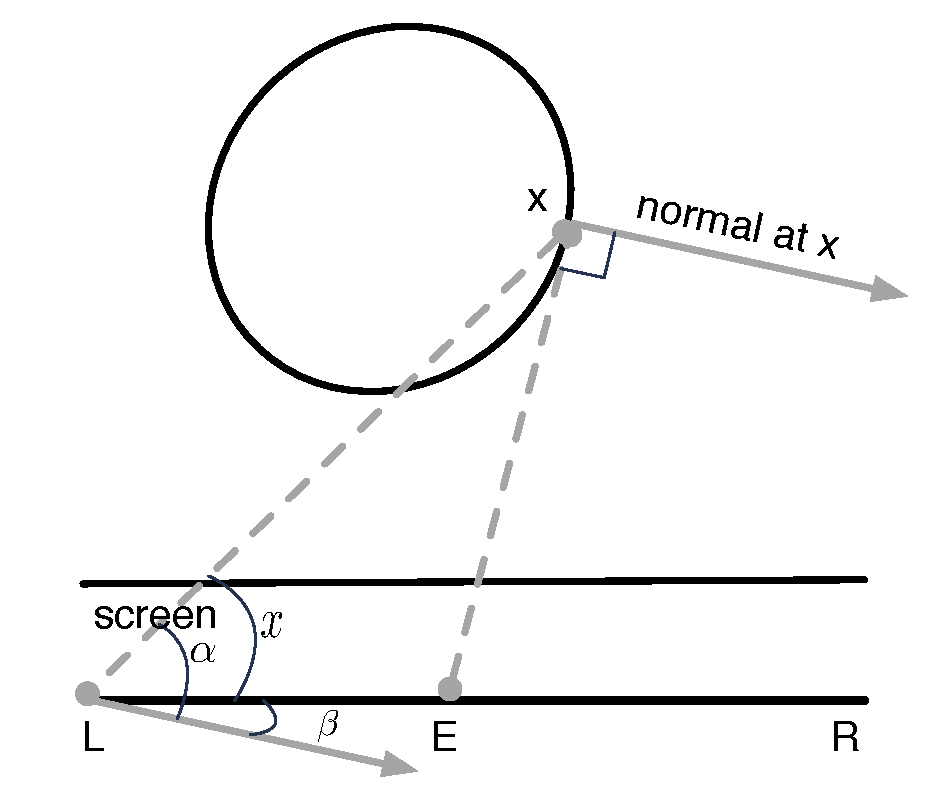
\includegraphics[width=0.6\linewidth]{deduction_t}
    \caption[轨迹函数的推导]{\label{fig:deduction_t}
    $t$的导数的推导}
\end{figure}  

首先,$x$的位置$P(x)$的导数的方向正是该点的切线方向,换言之,$P'(x)$与法线方向垂直。因此有以下公式:

\begin{equation}\label{eq:perp}
    P'\cdot{N} = 0
\end{equation}

\begin{figure}[bth]
    \centering
    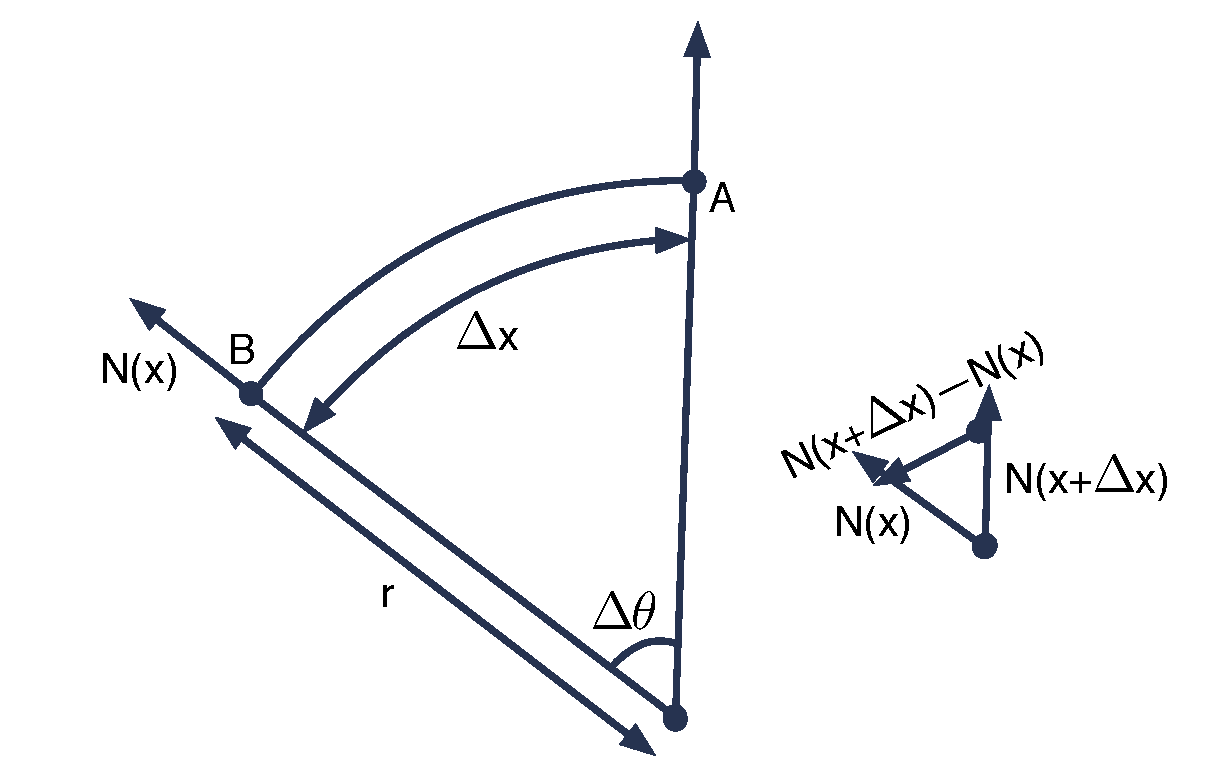
\includegraphics[width=0.6\linewidth]{deduction_n}
    \caption[曲线的法线导数的推导]{\label{fig:deduction_n}
    曲线的法线导数的推导}
\end{figure}

再者,$x$的法线方向$N(x)$的导数可以进行以下的推导得出。首先,$N(x)$可以作为单位法线使用,原因如下:

\begin{equation}
    t_c = \frac{(P-L)\cdot{N}}{(R-L)\cdot{N}} = \frac{(P-L)\cdot{\frac{N}{|N|}}}{(R-L)\cdot{\frac{N}{|N|}}}
\end{equation}

接着,正如\autoref{fig:deduction_n}所示,当$P(x+\Delta x)$从$A$移动到$B$,$N(x)$,$N(x+\Delta x)$和$N(x+\Delta x)$ - $N(x)$组成来一个等腰三角形,因为$N(x)$和$N(x+\Delta x)$都是单位法线。因此可以得出:

\begin{equation}
    |N(x+\Delta x) - N(x)| = \Delta\theta \cdot 1 = \Delta\theta = |N'(x)\Delta x|
\end{equation}

又由于$\Delta x \to 0$,所以

\begin{equation}\label{eq:curvature}
    |N'(x)| = \lim_{x \to 0}\frac{\Delta\theta}{\Delta x} = \lim_{x \to 0}\frac{\Delta\theta}{r\Delta\theta} = \frac{1}{r} = C(x)
\end{equation}

其中$C(x)$表示\ec{}上一点$x$的曲率。另外,当$\Delta x \to 0$,$|N(x+\Delta x) - N(x)|$的方向趋近于与法线$N(x)$的方向垂直,因此可以得到$N'(x) \perp N(x)$。假设 $\alpha$表示$P(x)-L$和$N(x)$之间的夹角,$\beta$表示$R-L$和$N(x)$之间的夹角,可以进行如下的转化:

\begin{equation}\label{eq:alpha}
(P-L)\cdot{N'} = |P-L|{|N'|}\cos{(\alpha+\frac{\Pi}{2})} = |P-L|{|N'|}\sin\alpha
\end{equation}

\begin{equation}\label{eq:beta}
(R-L)\cdot{N'} = |R-L|{|N'|}\cos{(\beta+\frac{\Pi}{2})} = |R-L|{|N'|}\sin\beta
\end{equation}

结合\autoref{eq:derivative},\autoref{eq:perp},\autoref{eq:curvature},\autoref{eq:alpha}和\ref{eq:beta},可以得到:

\begin{equation}\label{eq:final}
\begin{split}
t_c' & = \frac{C|P-L||N|\sin\alpha|R-L||N|\cos\beta-C|R-L||N|\sin\beta|P-L||N|\cos\alpha}{((R-L)\cdot{N})^2} \\
& = \frac{C|P-L||R-L||N|^2(\sin\alpha\cos\beta-\sin\beta\cos\alpha)}{((R-L)\cdot{N})^2} \\
& = \frac{C|P-L||R-L||N|^2\sin(\alpha-\beta)}{((R-L)\cdot{N})^2} \\
& = \frac{C|P-L||R-L||N|^2\sin(\gamma)}{((R-L)\cdot{N})^2}
\end{split}
\end{equation}

正如\autoref{fig:deduction_t}所示,$\gamma$是$P(x)-L$和$R-L$之间的夹角。由于$x$ 位于$L$与$R$连线的正前方,$sin\gamma$的值恒大于0。因此,$t_c'(x)$的符号只与$C(x)$有关。

需要明确指出的是,由于三维模型的不连续性,$t_c'(x)=0$在模型上出现的位置并不是连续的。因此,本文将通过$t_c'(x-)t_c'(x+) < 0$而不是$t_c'(x)=0$来找出极值点。

在本文设计的方法中,会将\ec{}上的\conp{}投影到左眼和右眼对应的图像,再沿着极线(epipolar line)而不是物体空间中的\ec{}(epipolar curve)进行搜索。这样一来,即可计算出极值点并存储到图像空间,从而在图像空间实现\epsl{}的判定。

\subsection{\scon{}}
\label{sec:suggestive_contour_math}
通过检测对应视点的轨迹的想法同样可以应用到\scon{}上。\scon{}的定义如下:

\begin{align}
  \kappa_r &= 0 \label{eq:Kr} \\
  D_w\kappa_r &> 0 \label{eq:DwKr} 
\end{align}

其中$\kappa_r$表示表面上一点的径向曲率,$D_w\kappa_r$表示$\kappa_r$的方向导数。更确切地说,$\kappa_r$是视线方向$V$在切平面上的投影$W$的方向上的法向曲率。法向曲率以及方向导数的概念已经在\autoref{sec:diff_geo}中进行说明,在此不再赘述。$\kappa_r$可以用以下形式表示为关于主曲率和$W$的函数:

\begin{equation}\label{eq:normal curvature}
    \kappa_r = \kappa_1cos^2\phi+\kappa_2sin^2\phi
\end{equation}

其中$\kappa_1$和$\kappa_2$是两个主曲率,$\phi$是$W$的方向与$\kappa_1$对应的主曲率方向(principal curvature direction)。为了找到\scon{}与视点之间的对应关系,将$\kappa_r = 0$代入\autoref{eq:normal curvature},并结合$cos^2\phi + sin^2\phi = 1$,可以得到:

\begin{align}
    cos^2\phi &= \frac{\kappa_2}{\kappa_2-\kappa_1} \label{eq:cos}\\
    sin^2\phi &= \frac{-\kappa_1}{\kappa_2-\kappa_1} \label{eq:sin}
\end{align}

从\autoref{eq:cos}和\autoref{eq:sin}中可以分别获知满足$\kappa_r = 0$的$W$与主方向$D_1$形成的夹角的余弦值和正弦值。于是,假设$\kappa_1$和$\kappa_2$满足$\kappa_1\kappa_2 \leq 0$,可以按照以下形式计算出满足$\kappa_r = 0$的$W$:

\begin{align}
    W &= cos{\phi}D_1+sin{\phi}D_2 \\
    &= \pm\sqrt{\frac{\kappa_2}{\kappa_2-\kappa_1}}D_1\pm\sqrt{\frac{-\kappa_1}{\kappa_2-\kappa_1}}D_2 \label{eq:w}
\end{align}

其中$D_1$和$D_2$是分别是对应的主曲率的方向。尽管\autoref{eq:w}中$\kappa_r = 0$的解有四个,但是由于视点$E$观察到的三维模型上的一点$x$必然位于$E$的前方,所以$\kappa_r = 0$的四个解中只有其中两个可以是$L$和$R$之间一个视点$E$的视线方向的投影(另外的两个解所代表的方向与这两个解代表的方向完全相反)。

\begin{figure}[tbp]
    \centering
    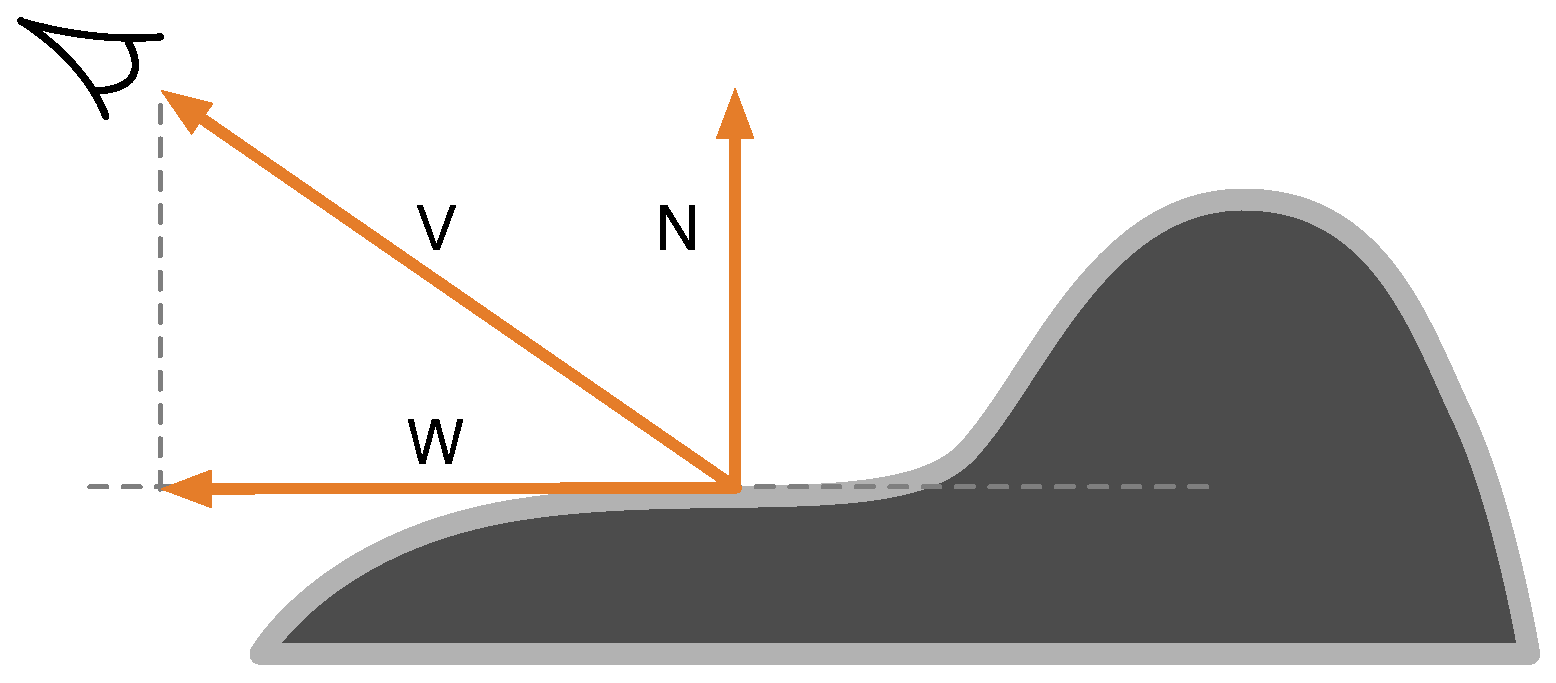
\includegraphics[width=0.9\linewidth]{suggestive_contour_definition}
    \caption[\scon{}的定义]{\label{fig:suggestive_contour_definition2}
    \scon{}的定义。其中$N$表示表面法线,$V$表示视线方向,$W$表示$V$在切平面上的投影。}
\end{figure}

至此,本文得出了将表面点$x$视为\sconp{}的$W$的表达式,但是还未建立将表面点$x$视为\sconp{}的视点$E$的与$x$上的几何特征所存在的直接关系。为了建立这一关系,需要回顾\autoref{fig:suggestive_contour_definition2}中展示的\scon{}的定义。由于$W$是$V$在切平面上的投影,所以在确定$W$后,$V$必须要位于$W$和$x$上的法线$N$形成的面内。换言之,假设将$W$和$x$上的法线$N$的叉积记为$M$:

\begin{equation}\label{eq:suggestive viewpoint}
    M = W \times N
\end{equation}

那么,视点$E$观察点$x$所形成的视线方向必定垂直于$M$。所以,将某个表面点视为\sconp{}的视点$E$必须满足:

\begin{equation}\label{eq:suggestive viewpoint}
    {(E - P)}\cdot{M} = 0
\end{equation}

不难看出,由于\autoref{eq:suggestive viewpoint}的形式和\autoref{eq:t1}一致,同样地,可以将视点$E$用一个参数$t$参数化成\autoref{eq:viewpoint1}的形式并推导出$t$的表达式:

\begin{equation}\label{eq:suggestive trajectory}
    t = \frac{(P-L)\cdot{M}}{(R-L)\cdot{M}}
\end{equation}

该公式表示了\scon{}的对应视点的轨迹函数,也就是$t_s(x)$。同样地,基于$t_s(x)$可以计算出极值点从而对\scon{}的\epsl{}进行判定。然而,与\con{}不同的是,对于每个\sconp{}会有两个对应的视点将其视为\sconp{},所以$t_s(x)$是一个多值函数(multivalued function)。关于\scon{}的极值点的计算细节将在\ref{sec:suggestive_contour_algorithm}中进一步阐述。

另外,关于$t_s(x)$的推导是建立在$\kappa_1\kappa_2 \leq 0$的假设的前提下的,如果$x$上的两个主曲率不满足$\kappa_1\kappa_2 \leq 0$,那么就不存在使$\kappa_r = 0$成立的方向$W$,也不存在对应的视点将$x$视为\sconp{}。

与$\kappa_1\kappa_2 \leq 0$类似,还有其他条件会使得不存在对应的视点将$x$视为\sconp{}。在上述的讨论中,\scon{}的另一个决定条件$D_w\kappa_r>0$还没有考虑在内。同样地,如果$x$上的径向曲率$\kappa_r$的方向导数不满足$D_w\kappa_r>0$,那么即使$x$能够找到满足$\kappa_r = 0$的对应视点,该点也不会被视为\sconp{}。

再者,在实际运用中,还会用以下的条件来进一步限制\scon{}的出现范围:

\begin{equation}\label{eq:cosNdotV}
  cos^{-1}(N\cdot{V}) > \theta_c 
\end{equation}

其中$\theta_c$是一个用户设定的常量。由于直接通过定义检测得到的\scon{}并不稳定,在画面上来看会随着视点和三维模型相对位置的变化而剧烈变化,造成画面闪烁、线条看起来不连续的现象。因此,在实际运用中会通过\autoref{eq:cosNdotV}中的条件来进一步对按照定义检测出的\scon{}进行筛选,去掉这些不稳定的部分的\sconp{}。

综上所述,对于那些不符合上述三个条件的表面点,不存在对应的视点将其视为\sconp{}。换言之,$t_s(x)$的区间端点有三种:

\begin{enumerate}
\item $\kappa_1\kappa_2 = 0$
\item $D_w\kappa_r = 0$
\item $cos^{-1}(N\cdot{V}) = \theta_c$
\end{enumerate}

满足上述三个条件之一的点都是$t_s(x)$的区间端点。除了极值点以外,这些区间端点也会破坏对应视点的轨迹的单调性。因此,对于\scon{}来说,要实现\epsl{}的判定,除了计算出极值点外,还需要计算出这些区间端点并将它们存储到\ppll{}。
% 在后续的图像空间搜索来判定\epsl{}时,这些区间端点的作用和极值点相同,都是判定\sconp{}不是\stc{}并停止搜索的依据。